\documentclass[tikz,border=2mm,svgnames]{standalone}

\tikzset{every picture/.append style={%
    scale=0.8,
}}

\begin{document}

% question
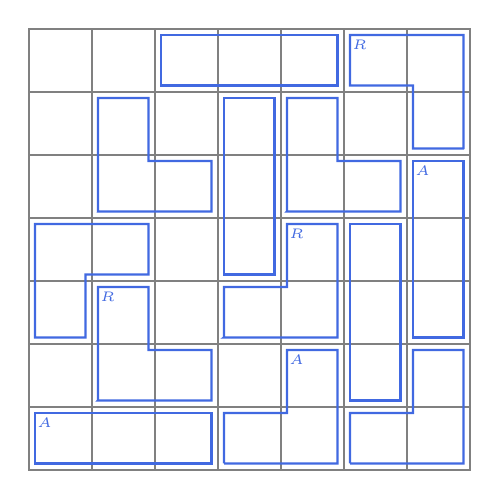
\begin{tikzpicture}
  % background grid
  \draw[line cap=rect, thick, gray] grid(7, 7);

  % annotations
  \node[RoyalBlue,font=\tiny] at(0+0.25,0+0.75){$A$};
  \node[RoyalBlue,font=\tiny] at(1+0.25,2+0.75){$R$};
  \node[RoyalBlue,font=\tiny] at(4+0.25,1+0.75){$A$};
  \node[RoyalBlue,font=\tiny] at(4+0.25,3+0.75){$R$};
  \node[RoyalBlue,font=\tiny] at(5+0.25,6+0.75){$R$};
  \node[RoyalBlue,font=\tiny] at(6+0.25,4+0.75){$A$};
 
  % rectangular boxes
  %\draw[RoyalBlue,thick] (0.1,0.1)-|(2.9,0.9)-|cycle;% alternative to rectangle
  \draw[RoyalBlue,thick] (0.1,0.1) rectangle (2.9, 0.9);
  \draw[RoyalBlue,thick] (2.1,6.1) rectangle (4.9, 6.9);
  \draw[RoyalBlue,thick] (3.1,3.1) rectangle (3.9, 5.9);
  \draw[RoyalBlue,thick] (5.1,1.1) rectangle (5.9, 3.9);
  \draw[RoyalBlue,thick] (6.1,2.1) rectangle (6.9, 4.9);

  % L-Shaped boxes
  \draw[RoyalBlue,thick] (0.1,2.1)-|(0.9,3.1)-|(1.9,3.9)-|cycle;
  \draw[RoyalBlue,thick] (1.1,1.1)-|(2.9,1.9)-|(1.9,2.9)-|cycle;
  \draw[RoyalBlue,thick] (4.1,4.1)-|(5.9,4.9)-|(4.9,5.9)-|cycle;
  \draw[RoyalBlue,thick] (3.1,0.1)-|(4.9,1.9)-|(4.1,0.9)-|cycle;
  \draw[RoyalBlue,thick] (5.1,0.1)-|(6.9,1.9)-|(6.1,0.9)-|cycle;
  \draw[RoyalBlue,thick] (3.1,2.1)-|(4.9,3.9)-|(4.1,2.9)-|cycle;
  \draw[RoyalBlue,thick] (1.1,4.1)-|(2.9,4.9)-|(1.9,5.9)-|cycle;
  \draw[RoyalBlue,thick] (6.9,5.1)-|(6.1,6.1)-|(5.1,6.9)-|cycle;
\end{tikzpicture}

% solution
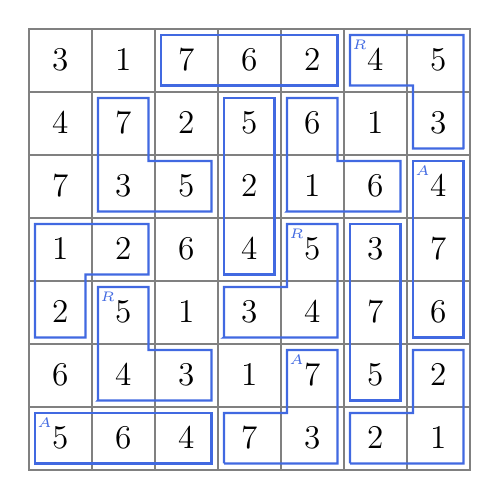
\begin{tikzpicture}
  % background grid
  \draw[line cap=rect, thick, gray] grid(7, 7);

  % annotations
  \node[RoyalBlue,font=\tiny] at(0+0.25,0+0.75){$A$};
  \node[RoyalBlue,font=\tiny] at(1+0.25,2+0.75){$R$};
  \node[RoyalBlue,font=\tiny] at(4+0.25,1+0.75){$A$};
  \node[RoyalBlue,font=\tiny] at(4+0.25,3+0.75){$R$};
  \node[RoyalBlue,font=\tiny] at(5+0.25,6+0.75){$R$};
  \node[RoyalBlue,font=\tiny] at(6+0.25,4+0.75){$A$};
 
  % rectangular boxes
  %\draw[RoyalBlue,thick] (0.1,0.1)-|(2.9,0.9)-|cycle;% alternative to rectangle
  \draw[RoyalBlue,thick] (0.1,0.1) rectangle (2.9, 0.9);
  \draw[RoyalBlue,thick] (2.1,6.1) rectangle (4.9, 6.9);
  \draw[RoyalBlue,thick] (3.1,3.1) rectangle (3.9, 5.9);
  \draw[RoyalBlue,thick] (5.1,1.1) rectangle (5.9, 3.9);
  \draw[RoyalBlue,thick] (6.1,2.1) rectangle (6.9, 4.9);

  % L-Shaped boxes
  \draw[RoyalBlue,thick] (0.1,2.1)-|(0.9,3.1)-|(1.9,3.9)-|cycle;
  \draw[RoyalBlue,thick] (1.1,1.1)-|(2.9,1.9)-|(1.9,2.9)-|cycle;
  \draw[RoyalBlue,thick] (4.1,4.1)-|(5.9,4.9)-|(4.9,5.9)-|cycle;
  \draw[RoyalBlue,thick] (3.1,0.1)-|(4.9,1.9)-|(4.1,0.9)-|cycle;
  \draw[RoyalBlue,thick] (5.1,0.1)-|(6.9,1.9)-|(6.1,0.9)-|cycle;
  \draw[RoyalBlue,thick] (3.1,2.1)-|(4.9,3.9)-|(4.1,2.9)-|cycle;
  \draw[RoyalBlue,thick] (1.1,4.1)-|(2.9,4.9)-|(1.9,5.9)-|cycle;
  \draw[RoyalBlue,thick] (6.9,5.1)-|(6.1,6.1)-|(5.1,6.9)-|cycle;

  % solution values
  % Row 1
  \node[font=\large\bfseries] at (0.5,0.5){$5$};
  \node[font=\large\bfseries] at (1.5,0.5){$6$};
  \node[font=\large\bfseries] at (2.5,0.5){$4$};
  \node[font=\large\bfseries] at (3.5,0.5){$7$};
  \node[font=\large\bfseries] at (4.5,0.5){$3$};
  \node[font=\large\bfseries] at (5.5,0.5){$2$};
  \node[font=\large\bfseries] at (6.5,0.5){$1$};
  % Row 2
  \node[font=\large\bfseries] at (0.5,1.5){$6$};
  \node[font=\large\bfseries] at (1.5,1.5){$4$};
  \node[font=\large\bfseries] at (2.5,1.5){$3$};
  \node[font=\large\bfseries] at (3.5,1.5){$1$};
  \node[font=\large\bfseries] at (4.5,1.5){$7$};
  \node[font=\large\bfseries] at (5.5,1.5){$5$};
  \node[font=\large\bfseries] at (6.5,1.5){$2$};
  % Row 3
  \node[font=\large\bfseries] at (0.5,2.5){$2$};
  \node[font=\large\bfseries] at (1.5,2.5){$5$};
  \node[font=\large\bfseries] at (2.5,2.5){$1$};
  \node[font=\large\bfseries] at (3.5,2.5){$3$};
  \node[font=\large\bfseries] at (4.5,2.5){$4$};
  \node[font=\large\bfseries] at (5.5,2.5){$7$};
  \node[font=\large\bfseries] at (6.5,2.5){$6$};
  % Row 4
  \node[font=\large\bfseries] at (0.5,3.5){$1$};
  \node[font=\large\bfseries] at (1.5,3.5){$2$};
  \node[font=\large\bfseries] at (2.5,3.5){$6$};
  \node[font=\large\bfseries] at (3.5,3.5){$4$};
  \node[font=\large\bfseries] at (4.5,3.5){$5$};
  \node[font=\large\bfseries] at (5.5,3.5){$3$};
  \node[font=\large\bfseries] at (6.5,3.5){$7$};
  % Row 5
  \node[font=\large\bfseries] at (0.5,4.5){$7$};
  \node[font=\large\bfseries] at (1.5,4.5){$3$};
  \node[font=\large\bfseries] at (2.5,4.5){$5$};
  \node[font=\large\bfseries] at (3.5,4.5){$2$};
  \node[font=\large\bfseries] at (4.5,4.5){$1$};
  \node[font=\large\bfseries] at (5.5,4.5){$6$};
  \node[font=\large\bfseries] at (6.5,4.5){$4$};
  % Row 6
  \node[font=\large\bfseries] at (0.5,5.5){$4$};
  \node[font=\large\bfseries] at (1.5,5.5){$7$};
  \node[font=\large\bfseries] at (2.5,5.5){$2$};
  \node[font=\large\bfseries] at (3.5,5.5){$5$};
  \node[font=\large\bfseries] at (4.5,5.5){$6$};
  \node[font=\large\bfseries] at (5.5,5.5){$1$};
  \node[font=\large\bfseries] at (6.5,5.5){$3$};
  % Row 7
  \node[font=\large\bfseries] at (0.5,6.5){$3$};
  \node[font=\large\bfseries] at (1.5,6.5){$1$};
  \node[font=\large\bfseries] at (2.5,6.5){$7$};
  \node[font=\large\bfseries] at (3.5,6.5){$6$};
  \node[font=\large\bfseries] at (4.5,6.5){$2$};
  \node[font=\large\bfseries] at (5.5,6.5){$4$};
  \node[font=\large\bfseries] at (6.5,6.5){$5$};
\end{tikzpicture}

\end{document}
